\graphicspath{{chapters/notes/06/images/}}
\chapter{Tumor evolution studies: copy number based methods}

\section{Analysis of clonality}

  \subsection{Informative SNPs}
  Informative SNPs are at the basis of tumour evolution studies.
  An informative SNP is a SNP for which a specific individual has an heterozygous call.
  The set of informative SNP is unique for each individual.
  The somatic loss of an allele of a genomic region that contains an informative SNP will change its allelic fraction.
  In this way the allelic fraction of that informative SNP will be informative of the lesion and of its depth.
  In this way clonality of the tumour will be determined by the fraction of tumour cells that harbour the lesion:

  \begin{multicols}{2}
    \begin{itemize}
      \item A set of lesions in a sample is said to be clonal when all tumour cells harbour it.
      \item A set of lesions in a sample is said to be subclonal when only a subpopulation of tumour cells harbour it.
    \end{itemize}
  \end{multicols}

  \subsection{Log2 ratio}
  The Log2 ratio is computed as:

  $$\log_2\frac{\# tumour\ content}{\# normal content}$$

  This measure can be obtained through the intensity of signals in array data or through the local coverage over a tumour BAM file over a normal one.
  The log2 ratio help to uncover the ploidy and copy number changes of the tumour population in a sample.
  In particular:

  \begin{multicols}{3}
    \begin{itemize}
      \item $\log_2 R<0$ loss of copy number in tumour.
      \item $\log_2 R=0$ the tumour is copy number neutral.
      \item $\log_2 R >0$ gain of copy number in tumour.
    \end{itemize}
  \end{multicols}

  \subsection{Beta value}
  The $\beta$ value is the percentage of neutral reads, or the number of reads that can be coupled, one with the reference base and one with the alternative, over the total number of reads at a SNP.
  $\beta$ is used to evaluate the purity of a sample.
  In particular:

  \begin{multicols}{2}
    \begin{itemize}
      \item When $\beta=1$ the purity of the sample is $0$, so there is no tumour content with copy-number variations and so no tumour signal.
      \item If $\beta=0$ the purity of the sample is $1$, so there is only tumour content with copy-number variations.
    \end{itemize}
  \end{multicols}

  It can be seen how, the more $\beta$ tends to $0$, the higher the tumour content and the clonality of the sample.

  \subsection{Cluster analysis in the beta-log2 ratio space}
  Figure \ref{fig:cluster0} is an example of a sample in which cells cluster in population in the $\log_2 R\times\beta$ space.

  \begin{figure}[H]
    \begin{tabular}{cc}
      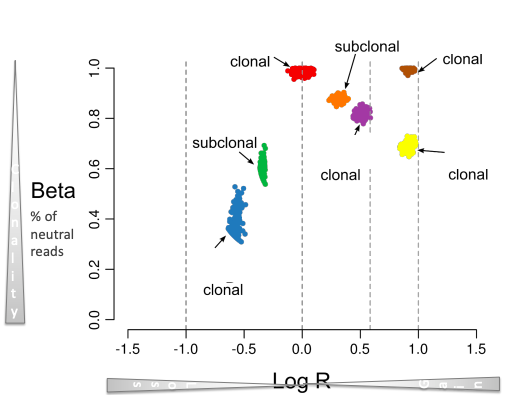
\includegraphics[width=0.5\textwidth]{image2.png} &   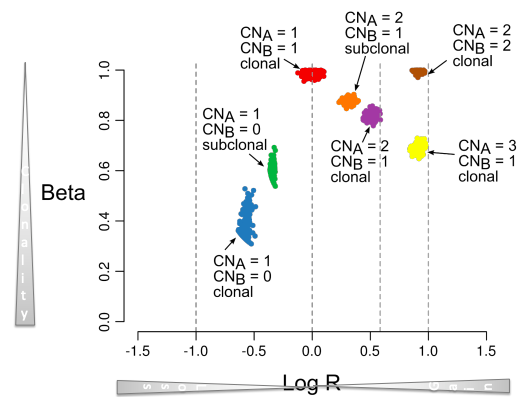
\includegraphics[width=0.5\textwidth]{image3.png} \\
    (a) Clonality & (b) CNV \\[6pt]
    \end{tabular}
    \caption{$\log_2 R\times \beta$ space of a tumour sample.}
    \label{fig:cluster0}
  \end{figure}

  Considering the $\beta$ value it can be said that lower clusters are more clonal, while considering the $\log_2 R$ value moving to the left side the more the cells have lost DNA, while moving to the right side the more the cells have gained DNA.
  Panel $A$ allow the visualization of the cluster, while panel $B$ adds information about the copy number changes of two specific alleles.
  The dotted lines are built in a data-driven manner and they represent events of deletion of gains for an allele.
  The informations that can be extrapolated from these graphs are:

  \begin{multicols}{2}
    \begin{itemize}
    \item The blue cluster with deletions is the most clonal one as it is the lower one.
    \item Both blue and green clusters have deletions, since they have a negative $\log_2 R$, but the green one is less clonal than the blue one as it is higher.
      It can be seen hot both the clusters have the same copy number for the two alleles, and ho they have lost a copy for one and both for the other.
    \item The red cluster is found in $\log_2 R = 0$ and $\beta = 1$, so the cells in it are wild-type in terms of copy-number changes the total number of alleles is the same to healthy cells.
    \item All the other clusters with a positive $\log_2 R$ had a gain of DNA.
    \end{itemize}
  \end{multicols}

  So, the $\log_2 R\times\beta$ space allow to map the status of clonality and the number of copies for a specific segment in the genome.

\section{Evolution maps}

  \subsection{Introduction}
  The information obtained on clonality can be used to build evolution maps.
  These maps are useful to track the evolution of a tumour over time with specific conditions like treatments.

  \subsection{Building an evolution map}
  An evolution map is represented by a graph where each node represents a lesion and each arc represents a timing relationship between lesions.
  To build one a number of samples from different individual are collected and all concomitant lesion within each sample are considered.
  Then:

  \begin{multicols}{2}
    \begin{itemize}
      \item For each sample an edge is drawn from a more clonal lesion to a more subclonal one, compiling a list of lesions.
      \item Then the number of times this relationship is found in different samples is counted.
      \item If the number of times an edge is observed deems it significant it is added to the graph, with a weight proportional to the significance of the relationship.
        The significance of the relationship depends on the number of observations and the total number of co-occurrences.
    \end{itemize}
  \end{multicols}

  So, it is assumed that the more clonal a lesion is, the earlier it appeared during tumour evolution.
  This is assumed only if this relationship is found in enough samples.
  In this way clonality is linked with time and an evolution graph can be built.

  \subsection{A toy example}
  The first thing to consider when building an evolution map is to look within each individual at concomitant deletion where one is subclonal to the other one.
  Figure \ref{fig:evolution} depicts a number of concurrent lesions in different samples.

  \begin{figure}[H]
    \begin{tabular}{cc}
      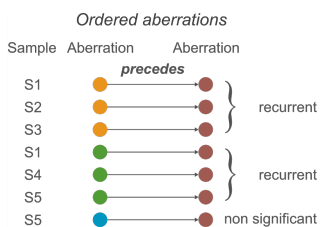
\includegraphics[width=0.5\textwidth]{image4.png} &   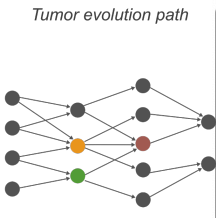
\includegraphics[width=0.5\textwidth]{image5.png} \\
    (a) Ordered aberration & (b) Tumour evolution path \\[6pt]
    \end{tabular}
    \caption{From ordered aberrations to a tumour evolution path.}
    \label{fig:evolution}
  \end{figure}

  Panel $A$ of the figure represents $5$ samples.
  The direction of the arrow indicates the subclonality of the lesions.
  From this panel it can be inferred that:

  \begin{multicols}{2}
    \begin{itemize}
      \item In samples $S1, S2$ and $S3$ the brown lesion is subclonal to the yellow one.
      \item In samples $S2, S4$ and $S5$ the brown lesion is subclonal to the green one.
      \item In sample $S5$ the brown lesion is subclonal to the blue one.
    \end{itemize}
  \end{multicols}

  So, from these it can be inferred that the yellow and green lesions preceded in the tumour evolution the brown one.
  The same cannot be said for the blue one as only one sample provides that information, making the statistical analysis non significant.
  Panel $B$ represent instead a graph of the tumour evolution path:

  \begin{multicols}{2}
    \begin{itemize}
      \item The yellow and the green lesions are on the same depth and they are not connected.
      \item The brown lesion is more deep than the yellow and green ones and an edge from them comes into it.
    \end{itemize}
  \end{multicols}

  From this it can be inferred than the green and yellow lesions are at the same time point and this subpopulation both were subject, later in time, to the brown lesion.

  \subsection{A real world data example}

  \begin{figure}[H]
    \centering
    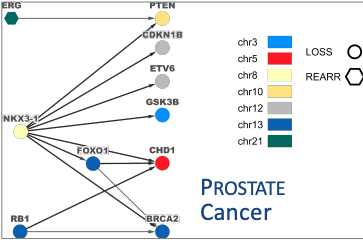
\includegraphics[width=0.5\linewidth]{image6.png}
    \caption{A tumour evolution graph built from real data}
    \label{fig:real}
  \end{figure}

  Performing this analysis all the dependencies supported by more than one individual can be considered.
  For example it has been found that in prostate cancer a loss in $NKX3$-$1$ precedes the deletion of $PTEN$.

    \subsubsection{Limitations}
    This type of studies are pretty limited: even with hundreds of whole exon sequencing data from large collections, the deepest graph had three layers.
    One reason for this is the harsh statistical requirements: two lesions must be co-occurrent and one must be subclonal to the other in a significant number of individual compared to the total number of individuals in which co-occurrence is found.
    The limiting factor is co-occurrence of the lesions.

  \subsection{Pathway-based evolutionary maps}
  To increase the ability to built this evolutionary maps single gene function information is aggregated into gene families or pathways.
  An example of this for prostate cancer is depicted in \ref{fig:prostate_path}.

  \begin{figure}[H]
    \centering
    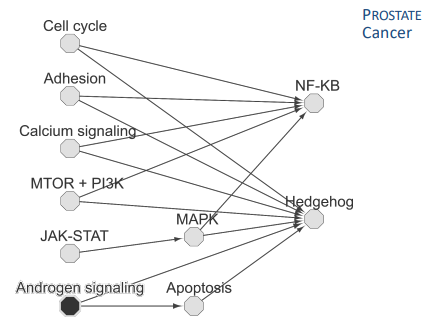
\includegraphics[width=0.4\linewidth]{pathways.png}
    \caption{Pathway evolution study example for prostate cancer}
    \label{fig:prostate_path}
  \end{figure}

  In this types of reconstructions, instead of considering lesions for a single genes, co-occurrences are counted including all the gene lesions with the same function in a pathway compared with lesion with the same function in another pathway.
  This method allow to have more data available to consider major changes during the evolution of the tumour pathway.
  So, a relationships between gene $B$ and gene $A$, and another between gene $C$ and gene $A$ can be assumed with the same effect and aggregated on the landing gene if $B$ and $C$ are from the same pathway.
  For example, considering PTEN, a tumour-suppressive gene relevant in pathway PF3K, all information that alter that pathway can be aggregated into one.
  In conclusion, in pathway-based evolutionary maps a set of pathways that are more or less altered at some level in earlier stages of the disease and that then trigger changes in other pathways are exploited.
  Doing so allow to learn more of the biology of the evolution of the disease.

    \subsubsection{Timing}
    There are also more complicated ways to make inference of tumor evolution.
    Some of this try to avoid the hypothesis that the more clonal a lesion is the more likely it is to happen early.
    This is because this is not always true: for example treatment could impair this process.

    \subsubsection{Treatment}
    In a treatment regiment, because of drug pressure selection, specific resistant clones harbouring a specific lesion can take over due to their higher rate of proliferation.
    In this case, a lesion that appears to be more clonal, could have happened later in time.
    It appears more clonal because of the higher proliferation rate due to an evolutionary advantage in resisting the treatment.

\section{Ploidy and purity corrections}

  \subsection{Introduction}
  To compare two different samples for which completely different levels of tumour content are quantified without having to convert every time and for every lesion the depth of the lesion based on tumour content there is a need to adjust the signal for tumour purity and ploidy.
  This is necessary also because the accuracy in calls for pure or admixed tissue with the same coverage is different and more false positive calls are likely in a more admixed sample.
  The coverage makes data coming from different samples comparable: everything is normalized to the total coverage, but this is not enough for diseased cells because of admixture.
  This necessity adds another step in data pre-processing and to do it it is necessary to know both tumour purity and ploidy.

  \subsection{A melanoma example}

  \begin{figure}[H]
    \centering
    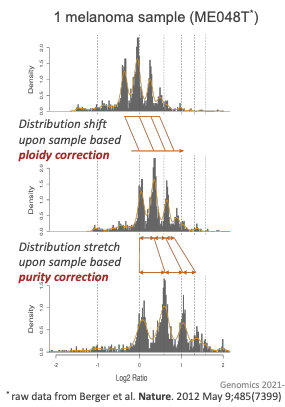
\includegraphics[width=0.4\linewidth]{image7.png}
    \caption{Highly aberrant melanoma sample: genome duplication and intervening lesions.}
    \label{fig:ploidy1}
  \end{figure}

  In figure \ref{fig:ploidy1} data from whole genome sequencing of one melanoma sample is depiced.
  Multiple peaks in the density of $\log_2 R$ correspond to different copy number states.
  Most of the time the best way to detect copy-number variants is to compare the tumour signals with the normal ones.
  Matching tumour data with no somatic changes to a normal genome the two samples will be similar and the histogram of the $\log_2 R$ will look like a normal distribution centred around $0$.
  A tumour sample with many heterozygous or homozygous deletions or copy-number gains will heave, other than the peak at $0$, two smaller peaks toward the left, with the first representing an heterozygous deletion and the second an homozygous one.
  Copy-number gains will be represented by peaks toward the right.
  Noise effect from admixture will make this secondary peaks difficult to distinguish, bringing them closer to $0$.

    \subsubsection{Ploidy correction}
    The ploidy is computationally assessed through the copy number space.
    In the example of \ref{fig:ploidy1} the first plot represents non-corrected data.
    Due to the genome duplication the main peak will not be in $0$, but more to the right.
    So, assessing the ploidy and looking at a backbone state of three copies for the genome, the main peak should be shifted to the right, as can be seen in the second graph.
    If instead, the tumour genome underwent more deletions, the signal will be moved to the left.
    In conclusion the distribution will be shifted toward zero.

    \subsubsection{Purity correction}
    Tumour admixture is computed and used to correct the graph.
    As tumour admixture dilutes the signal coming from the tumour, correcting for purity will stretch the peaks, making them more distant and easily obtainable.
    This can be seen in the last plot of \ref{fig:ploidy1}.

  \subsection{A melanoma example considering more samples}
  Global copy number changes will shift the peak of the distribution away from zero, while local ones will create different peaks in the distribution.
  Admixture will compress the distribution around its centre.
  In figure \ref{fig:ploidy2} an example is shown for $25$ samples of an highly aberrant melanoma tumour.

  \begin{figure}[H]
    \centering
    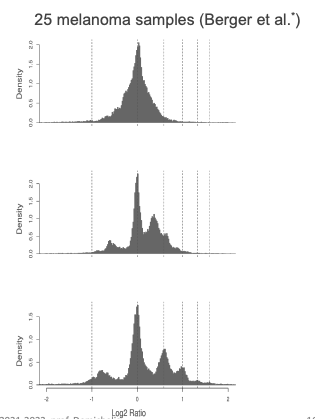
\includegraphics[width=0.4\linewidth]{image8.png}
    \caption{25 melanoma samples. With ploidy correction the signals start being interpretable, and with purity correction, while not perfect they become clear.}
    \label{fig:ploidy2}
  \end{figure}

  In the first graph in the figure it is represented the distribution of the $\log_2 R$ data of uncorrected signal.
  Every melanoma sample is highly aberrant with ploidy and purity different between individuals.
  The data is corrected to get rid of the noise.
  In the second graph data is corrected for ploidy, while in the third for both ploidy and purity.
  From the corrected data it is inferable that:

  \begin{itemize}
    \item A lot of tumours have a backbone ploidy of $2.$
    \item There are some homozygous deletion not perfectly centred in $1$ but closer to that value after the correction.
    \item Some signal is compatible with an homozygous deletion.
    \item A reasonable amount of signal for three copies is present: some tumours could have a threeploid status.
  \end{itemize}

  \subsection{An example with TGCA data}
  In this study data from TGCA was analysed to see how suboptimal tumour purity affect proper copy number data analysis and how common it is that purify is not $100\%$ and ploidy is not $2$ in the primary disease.

  \begin{figure}[H]
    \centering
    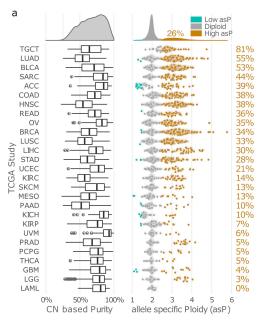
\includegraphics[width=0.5\linewidth]{image9.png}
    \caption{Tumour types and purity,}
    \label{fig:tcga}
  \end{figure}

  Figure \ref{fig:tcga} depicts a list of tumour types, where every line is a tumour type.
  On the $x$-axis tumour purity is depicted and for each type of tumour its distribution id depicted.
  Every tumour type has a different number of sample profiles.
  The middle vertical line represent the median signal of the distribution, the black horizontal line represent the interquartile range and some outlier are shown.
  Altogether, $8183$ primary cancer samples matched to $27$ tumour types profiled with WES from TCGA.
  $4,950$ cases with overall high tumour cellularity were identified.
  The majority had $69\%$ tumor purity.
  There are some outliers: for example ovarian cancer has high purity.

    \subsubsection{Ploidy correction}
    Considering ploidy there is a need to investigate what is the fraction within each tumour type with a ploidy significantly above $2.$
    In the plot the tumour types are sorted by decreasing percentage of tumours with a ploidy higher than $2$.
    For example for the first two types more than $50\%$ of the primary tumours have a ploidy status over $2$.
    This mean that either they underwent whole genome duplication or they have a triploidy status.
    Some tumours have very low ploidy: at least one of the copy of the genome is lost and there is low allele specific ploidy assessment.
    Figure \ref{fig:ploidy_tcga} shows the change of data distribution when the samples are corrected for ploidy and purity.

    \begin{figure}[H]
        \centering
        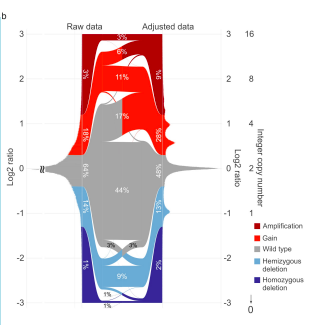
\includegraphics[width=0.5\linewidth]{image10.png}
        \caption{The $y$ axis is the $\log_2 R$. On the left raw data are represented, while on the right the adjusted ones.}
        \label{fig:ploidy_tcga}
    \end{figure}

    Focusing on the first half of the graph it can be seen how there is noise similar for the melanoma uncorrected data.
    The correction of the data resulted in the reclassification of $30\%$ of the totality of the segments.
    The correction led to the doubling of the observed homozygous deletions, meaning that the total number of unavailable protein products weren't being produced.

\section{Allele-specific analysis}

  \subsection{Introduction}
  Once tumour data has been corrected for purity and polity there is still a need to analyse allele specific information.
  Some allele could produce a non functional protein, or there could be copy-number neutral events.
  These aberration wouldn't be uncovered by the analysis done until now, so there is a need to add a step to evaluate them and their functional effects.

  \subsection{An example}
  \begin{figure}[H]
    \centering
    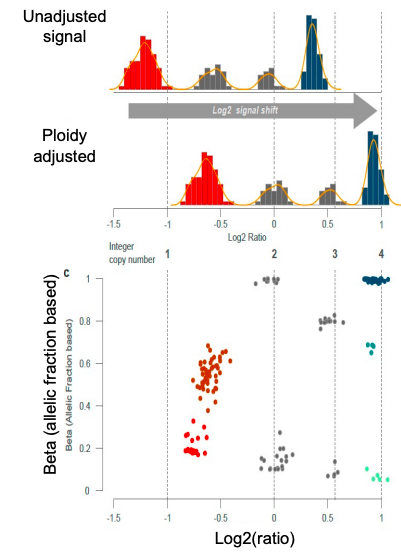
\includegraphics[width=0.5\linewidth]{image11.png}
    \caption{Top panel: loss of an allele on A so we'll have 2-1-2 copies. Bottom panel: same situation on allele A but allele B is doubled so we'll have 3-2-3 copies. So, in this situation, the gene x will have two copies but both of them coming from the same allele (B).\\
      By computing the log2 ratio in this situation we'll have the log2(2/2) which will lead to the collocation on the 0 axis but on the lower part (due to the clonality).}
    \label{fig:img11}
  \end{figure}

  Figure \ref{fig:img11} represents adjusted data for some samples.
  Then those samples are represented in the $\log_2 R\times\beta$ space.
  It can be seen how data underneath the peaks belong to specific clusters.
  This suggests how looking only at the $\log_2 R$ the presence of clusters with different clonalities is undetectable.
  The lower cluster with $\log_2 R = 0$ only one allele is visible, so there is a copy neutral loss of heterozygosity or CN-LOH: there are two copies of one allele and zero of the other.
  This becomes visible from the $\log_2 R\times \beta$ space: some equations allow to extrapolate the number of copies for each allele, as depicted in \ref{fig:img12}.

  \begin{figure}[H]
    \centering
    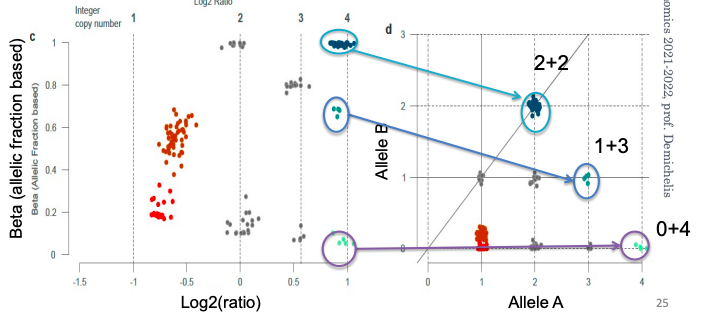
\includegraphics[width=0.5\linewidth]{image12.png}
    \caption{From $\log_2 R\times \beta$ space to allele-specific analysis}
    \label{fig:img12}
  \end{figure}

  It can be seen how for $2$ different allele and a copy number of $4$ there are three different combinations:

  \begin{itemize}
    \item $2$ copies of $A$ and $2$ copies of $B$.
    \item $3$ copies of $A$ and $1$ copy of $B$.
    \item $4$ copies of $A$ and $0$ copies of $B$.
  \end{itemize}

    \subsubsection{Changes of copy number for specific alleles}
    So it can be seen how once the data has been corrected for ploidy and purity the analysis can be shifted to the level of the number of copies of each allele for each gene.
    This is important because some alleles don't produce a functional protein, so in case when only them are present the function will still be lost, even with an allele present.
    Distinguishing the alleles is fundamental in distinguishing a possible loss of function.

    \begin{figure}[H]
      \centering
      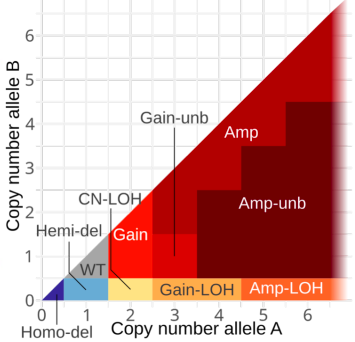
\includegraphics[width=0.3\linewidth]{image13.png}
      \caption{Effect of changes of copy number for specific alleles.}
      \label{fig:img13}
    \end{figure}

    \subsubsection{Copy number neutral events}
    This analysis allow to reclassify copy number status in the $\log_2 R\times \beta$ space and assign an allele-specific copy number to every segment of the genome, or to every gene.
    In this way a significant fraction of the genome that would appear wild-type for the copy number underwent loss of one allele and gain of the other.
    This event is called copy-neutral loss of heterozygosity or CN-LOH.
    A relevant fraction of high copy number levels from the TGCA data seen before came from the same allele.

    \begin{figure}[H]
      \centering
      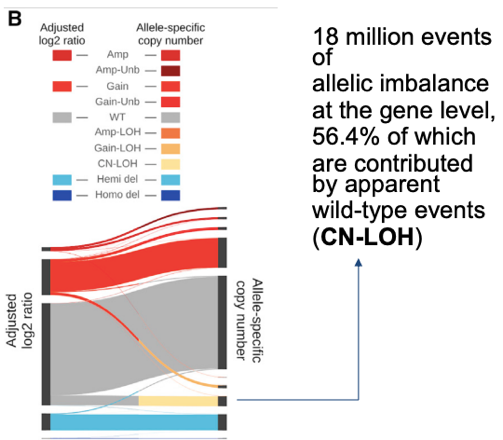
\includegraphics[width=0.5\linewidth]{image14.png}
      \caption{Ciani et al, Cell Syst 2022}
      \label{fig:img14}
    \end{figure}

    So, allele analysis is fundamental to get all the information necessary for a functional analysis of the genome.
    This information is relevant in precision medicine because there are ways to target genes exploiting loss of heterozygosity and this pipeline allow to discover this event even in the case of a wild type segment in term of copy number.

  \subsection{A case study}
  In the example depicted in \ref{fig:img15} data from a patient's primary and metastasis sample regarding the copy number for the alleles of sequenced genes are visible.

  \begin{figure}[H]
    \centering
    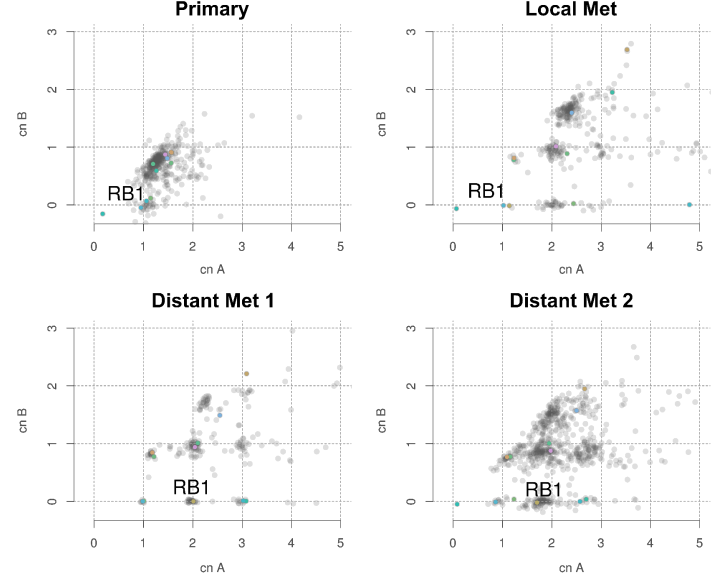
\includegraphics[width=0.7\linewidth]{image15.png}
    \caption{Copy number of $CN_A$ and $CN_B$ from multi-sample data from the same patient.}
    \label{fig:img15}
  \end{figure}

    \subsubsection{Primary site}
    In the primary site is visible that:

    \begin{multicols}{2}
      \begin{itemize}
        \item A cloud of dots has a total copy number of two $(1,1),(2,0),(0,2)$.
        \item A cluster underwent hemizygous deletion and only one copy is visible $(1,0),(0,1)$.
        \item A gene that underwent an homozygous deletion is visible $(0,0)$.
      \end{itemize}
    \end{multicols}

   \subsubsection{Metastasis}
    Other than the primary sites a local and two distance metastasis has been sequenced.
    From the data of those it can be seen how:

    \begin{multicols}{2}
      \begin{itemize}
        \item In distant met $1$ there are no homozygous deletion, so probably this metastasis happened before the deletion in the primary site.
        \item In both the distant metastasis $RB1$ gained an extra copy of allele $A$.
        \item In all the metastasis there are extra gains of copies of all the genes, so maybe a whole genome duplication happened.
        \item In distant met $1$ it can be seen how the data point in yellow are subclonal: they are close enough to $(1,1)$ that purity shifted them from $(1,0)$.
        \item Extra copies of the whole genome are likely in the local metastasis after the loss of the second copy of $RB1$.
        \item There is a copy number neutral loss of heterozygosity for many genes, including $RB1$.
        \item The level of subclonality is overall not high.
      \end{itemize}
    \end{multicols}


\section{Longitudinal plasma profiling}
Another way to track tumour evolution is to have data of the genomic landscape from different time points.

  \begin{figure}[H]
    \centering
    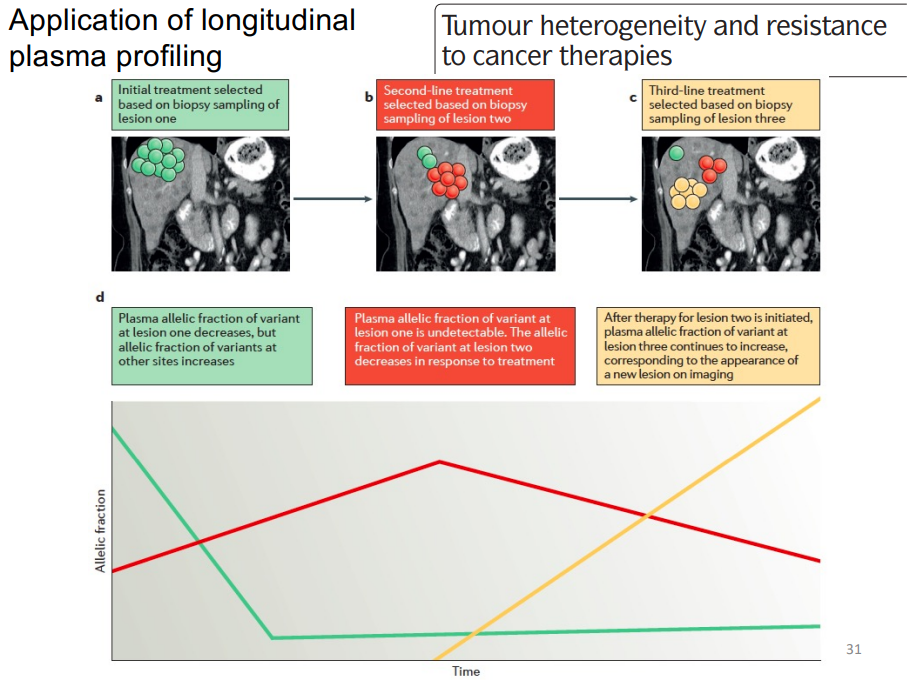
\includegraphics[width=0.8\linewidth]{image16.png}
    \caption{Application of longitudinal plasma profiling.}
    \label{fig:img16}
  \end{figure}

Longitudinal monitoring of alterations in circulating tumour DNA has the potential to enable molecular relapses to be detected before the emergence of disease relapse on imaging.

  \subsection{An example}
  In the hypothetical example depicted in figure \ref{fig:img16}.
  A biopsy sample from lesion $1$ in green leads to the use of a targeted agent directed at the alterations in lesion one (a).
  A failure to also lesion $2$ in red might then lead to outgrowth of clones harbouring alternative molecular alterations, prompting the use of a combination of targeted agents or use of a single targeted therapy capable Of overcoming both molecular alterations (b).
  The emergence Of lesion three in yellow might then be missed by biopsy sampling until this lesion becomes detectable on imaging (c).
  Longitudinal analysis of liquid biopsy Samples would enable the detection and determination of the allelic fractions of the variants at all three lesions before their detection on imaging (d).
  The figure illustrates the ability of the molecular analysis of plasma to convey the full spectrum of resistance alterations and shows the dynamic nature of resistance.

  \subsection{Tracking evolution}
  Dealing with biopsies over time the evolution of the disease can be tracked using the allelic fraction of a lesion.
  Naturally, these allelic fractions at any time point needs to be corrected for tumour content, otherwise different time points would be incomparable.
